% article example for classicthesis.sty
\documentclass[10pt,a4paper]{article} % KOMA-Script article scrartcl
\usepackage{import}
\usepackage{xifthen}
\usepackage{pdfpages}
\usepackage{transparent}
\newcommand{\incfig}[1]{%
    \def\svgwidth{\columnwidth}
    \import{./figures/}{#1.pdf_tex}
}
\usepackage{lipsum}     %lorem ipsum text
\usepackage{titlesec}   %Section settings
\usepackage{titling}    %Title settings
\usepackage[margin=10em]{geometry}  %Adjusting margins
\usepackage{setspace}
\usepackage{listings}
\usepackage{amsmath}    %Display equations options
\usepackage{amssymb}    %More symbols
\usepackage{xcolor}     %Color settings
\usepackage{pagecolor}
\usepackage{mdframed}
\usepackage[spanish]{babel}
\usepackage[utf8]{inputenc}
\usepackage{longtable}
\usepackage{multicol}
\usepackage{graphicx}
\graphicspath{ {./Images/} }
\setlength{\columnsep}{1cm}

% ====| color de la pagina y del fondo |==== %
\pagecolor{black}
\color{white}



\begin{document}
    %========================{TITLE}====================%
    \title{{  Solucion Taller 1 Análisis de Datos  }}
    \author{{Rodrigo Castillo}}
    \date{\today}

    \maketitle


     % ====| Loguito |==== %
    
\includegraphics[width=0.1\linewidth]{negro_cara.png}
    %=======================NOTES GOES HERE===================%
    \section{Las siguentes son 5 medidas sobre las variables $ x_1 , x_2 , x_3   $ }
        \begin{figure}[h!]
            \centering
            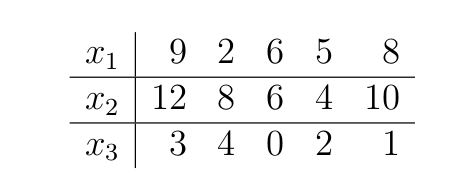
\includegraphics[width=0.5\linewidth]{punto1.png}
            \caption{Punto1}
            \label{fig:punto1}
        \end{figure}
        encuentre las matrices $ \hat{x} (vector de medias),  S_n 0 (mariz_{covarianzas})$  y $ R(matriz_{correlaciones})  $

    \section{Las 10 empresas mas grandes a nivel mundial producen los siguientes datos :}
        \begin{figure}[h!]
            \centering
            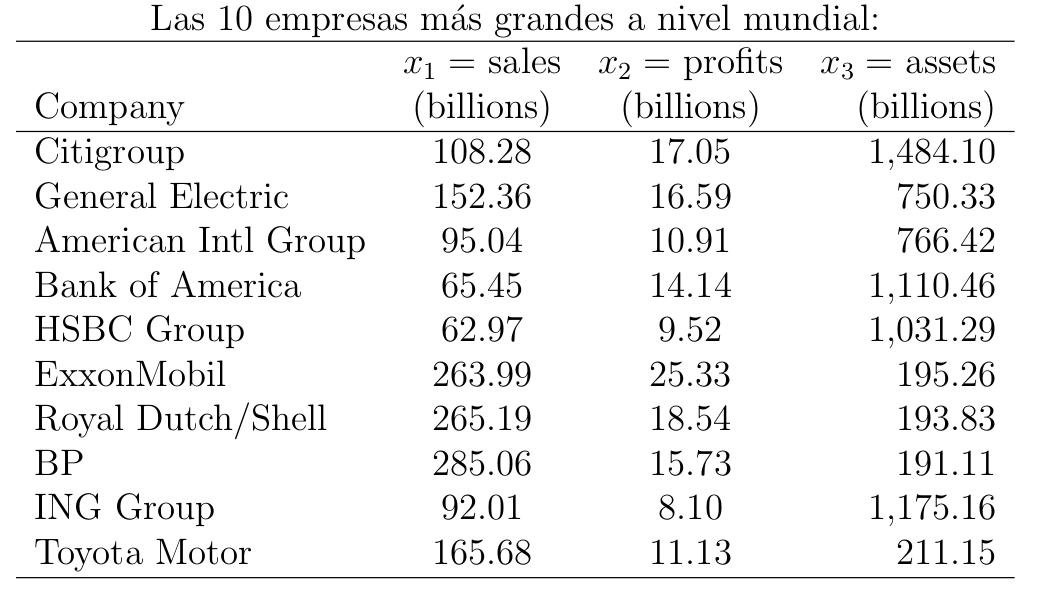
\includegraphics[width=0.5\linewidth]{datos.png}
            \caption{Datos}
            \label{fig:datos}
        \end{figure}

        \subsection{Grafique el diagrama de dispersión para las variables $ x_1
        $  y $ x_2   $ . Comente la apariencia del diagrama}

        \subsection{Calcule $ \hat{x_1}  , \hat{x_2}  , \hat{s_{11}}  ,
        \hat{s_{22}}  , \hat{s_{12}}   $  y $ r_{12}  $ }

        \subsection{Calcule $ \hat{x_1} , \hat{x_2}  , s_{11} , s_{22} , s_{12} ,
        r_{12}   $  y interprete $ r_{12}  $ }

        \subsection{Grafique los diagramas de dispersion para $ (x_2 , x_3 )  $
        y para $ (x_1 , x_3 )  $  Comente acerca de los patrones en ambas
        gráficas}

        \subsection{Calcule las matrices $ \hat{x}  , S_n    $ , $ R  $ para $
        (x_1 , x_2 , x_3 )  $   }

    \section{Dados los siguientes pares de medidas sobre dos variables $ x_1  $
    y $ x_2   $  }
        \begin{figure}[h!]
            \centering
            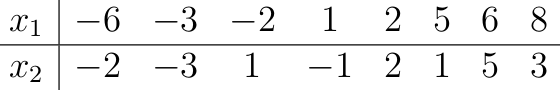
\includegraphics[width=0.5\linewidth]{fig.png}
            \caption{Punto 3}
            \label{fig:fig}
        \end{figure}

        grafique los datos como un diagrama de dispercion y calcule $ s_{11}
        ,s_{22} , s_{12}  $
        \\ Usando $ \hat{x_1}  = x_1 \cos{\theta } + x_2 \sin{\theta }   $  y $
        \hat{x_2}  = -x_1 \sin{\theta } + x_2 \cos{\theta }   $  calcule las
        medias correspondientes sobre las variables $ \hat{x_1}  , \hat{x_2 }
        $ asumiendo que los ejes coordenados originales están rotados en un
        angulo de $ \theta  = 26  $ \\
































    %=======================NOTES ENDS HERE===================%

    % bib stuff
    \nocite{*}
    \addtocontents{toc}{{}}
    \addcontentsline{toc}{section}{\refname}
    \bibliographystyle{plain}
    \bibliography{../Bibliography}
\end{document}
